\documentclass[]{article}
\usepackage[T1]{fontenc}
\usepackage[icelandic]{babel}
\usepackage{lipsum}
\usepackage{natbib}

\input{../shorthandCommon}

%opening
\title{Vélabrögð}
\author{Helga Ingimundardóttir}

\begin{document}

\maketitle

%\begin{abstract}\end{abstract}

\section{Inngangur}
Í stuttu máli snýst verkefnið um að læra að bera kennsl á góðar lausnir. 
Ég hef einskorðað verkefnið við tilviksrannsókn á verkniðurröðun á vélum (JSP, 
e. job-shop scheduling problem) 
sem felst í því að þurfa að gera raðbundnar ákvarðanir um hvaða verkefni eigi 
að vera afgreitt næst, þar sem þau eru að keppast um sömu aðföngin.
Í raun má útvíkka aðferðafræðina til hvers kyns strjála bestun. 

Hugmyndina að rannsókninni kviknaði þegar ég var að vinna í raunhæfu verkefni í 
aðgerðagreiningu í grunnnámi mínu. Um var að ræða bestun á verkniðurröðun fyrir 
Össur. Í eðli sínu er verkniðurröðun einfalt verkefni, og skipar stóran sess 
hjá framleiðslufyrirtækjum en stærðargráðan á vandamálinu gerir það að verkum 
að oft er erfitt að leysa verkefnið með nákvæmum aðferðum. 
Þetta voru mín fyrstu kynni af því að þurfa að sætta mig við einhverja lausn 
sem var ekki endilega hin fræðilega ,,besta'' lausn. 
Hér koma brjóstvitsaðferðir (e. heuristics) eða ,,þumalputtareglur'' sterkar 
inn, en þá er stóra spurningin hvernig má koma á sjálfvirkni í því ferli?

\section{Verkniðurröðun á vélar}
Gerum ráð fyrir að við höfum $n\times m$ JSP, 
þar sem $n$ verk, $\mathcal{J}=\{J_j\}_{j=1}^n$, 
eiga að vera afgreidd á $m$ vélum, $\mathcal{M}=\{M_a\}_{a=1}^m$. 
Verkefnin þurfa að vera afgreidd í tiltekinni röð, þ.e. sérhvert verk $J_j$ 
þarf að fylgja runu af $m$ aðgerðum 
$\vsigma_j=\{\sigma_{j1},\sigma_{j2},\dotsc,\sigma_{jm}\}$. 
Rétt er að taka fram að verk getur ekki hafist handa á næstu vél fyrr en það 
hefur lokið núverandi aðgerð. 
Þar að auki getur sérhver vél aðeins meðhöndlað eitt verk í einu. 
Viðbættar skorður sem eru oft teknar til greina eru sleppitími og útgáfutími, 
en þeir eru ekki til skoðunar hér.
Markfallið er að tímasetja öll verk þannig að lágmarka hámarks heildartíma (e. 
makespan), $C_{\max}$. 

\begin{figure}[p]\centering
    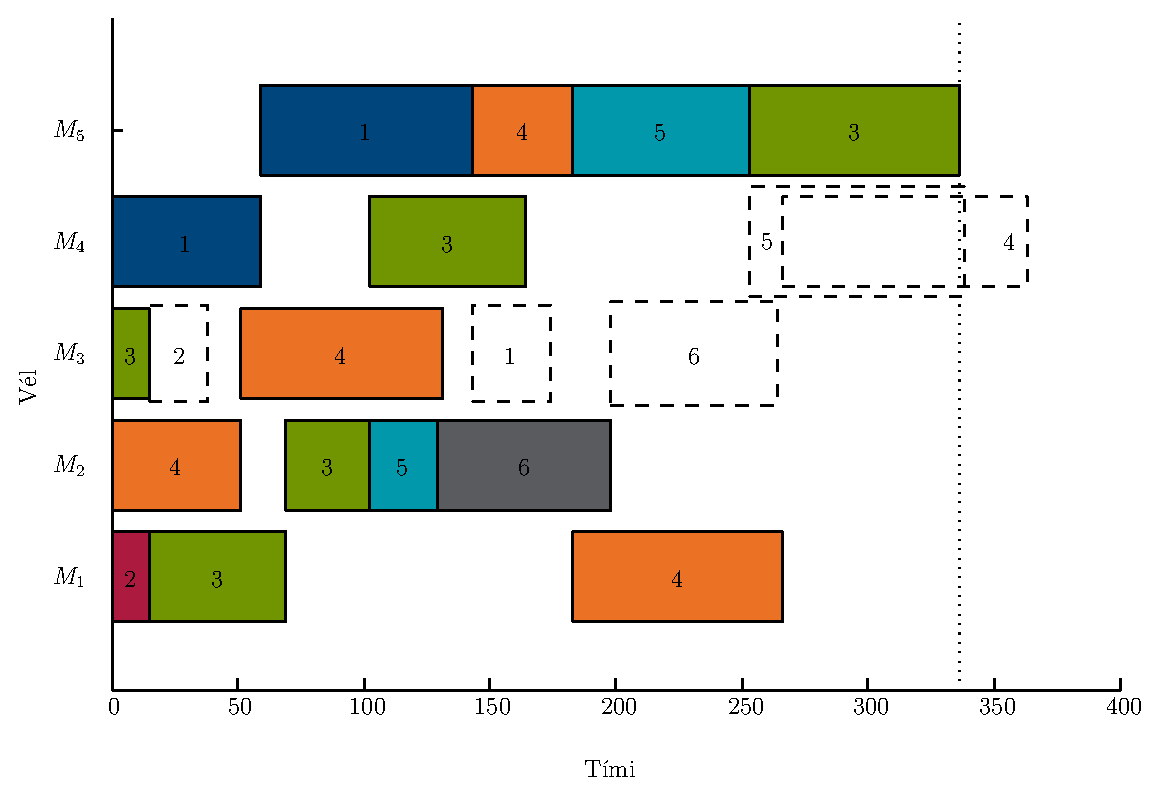
\includegraphics[width=0.8\textwidth]{figures/jssp_example.eps}
    \caption[Gantt rit af ókláraðri JSP stundaskrá]{Gantt rit af ókláraðri JSP 
    stundaskrá eftir 15 aðgerðir: heilir kassar tákna $\vchi$ og kassar með 
    brotalínu tákna $\mathcal{L}^{(16)}$. 
    Núverandi heildartími, $C_{\max}$, er gefinn upp sem brotalína.}
    \label{fig:jssp:example}
\end{figure}

Brjóstvitsaðferðir fyrir tímaáætlanir eru yfirleitt uppbyggingar- eða 
umbætunaralgrím.
Umbætunaralgrím byrja á fulbúinni lausn og reynir að finna sambærilegar, en 
betri lausnir. 
Uppbyggingaralgrím byrja með tóma lausn og bæta við einu verki í einu þar til 
lausnin er fullbúin, og er það sem aðferðafræðin gengur út frá. 
Í þessu tilfelli þá eru yfirleitt röðunarreglur 

The work presented here will focus on construction heuristics, although the 
techniques developed could be adapted to improvement heuristics also.  In 
scheduling a construction heuristic is typically implemented as a priority 
dispatching rule.  These are simple rules that basically determine which 
uncompleted job should be dispatched next.  However, knowing which job to 
dispatch is not sufficient, one must also know where to place it.  In order to 
build tight schedules it would be sensible to place the jobs, once they become 
available, such that the machine idle time is minimal. There may also be a 
number of different options for such a placement.
\Cref{fig:jssp:example} illustrates the dispatching process with an example of 
a temporal partial schedule for six jobs scheduled on five-machines.  The 
numbers in the boxes represent the job's identification $j$.  The width of the 
box illustrates the processing times for a given job for a particular machine 
$M_a$ (on the vertical axis).  The dashed boxes represent the resulting partial 
schedule for when a particular job is scheduled next.  Moreover, the current
$C_{\max}$ is denoted with a dotted horizontal line.  In the figure one observes
that $J_2$, to be scheduled on $M_3$, could be placed immediately in a slot 
between $J_3$ and $J_4$, or after $J_4$.  If $J_6$ had been scheduled prior a 
slot would have been created between it and $J_4$, thus creating a third 
alternative where $J_2$ is placed after $J_6$.  The construction heuristic must 
therefore decide where to place the job, and this may be independent of the 
dispatching rule applied.  Different placement strategies could be considered, 
for example placing a job in smallest feasible slot.  In our preliminary
experiments we have discovered that such a placement could rule out the 
possibility of constructing solutions with an optimal makespan. This problem 
did not occur when jobs were simply placed as early as feasibly possible.

A \emph{sequence} will refer to the sequential ordering of the dispatches of 
tasks to machines, i.e., $(j,a)$; the collective set of allocated tasks to 
machines, which is interpreted by its sequence, is referred to as a 
\emph{schedule}; a \emph{scheduling policy} will pertain to the manner in which 
the sequence is determined.  As shown in our example given in 
\Cref{fig:jssp:example}, there are 15 operations already scheduled. The 
sequence used to create the schedule was,
\begin{eqnarray}
\vchi=\left(J_3,J_3,J_3,J_3,J_4,J_4,J_5,J_1,J_1,J_2,J_4,J_6,J_4,J_5,J_3\right)
\end{eqnarray}
hence the current available jobs to be scheduled 
$\mathcal{L}=\{J_1,J_2,J_4,J_5,J_6\}$, and will be referred to as our job-list, 
describes the 5 potential jobs to be dispatched at step $k=16$ (note that $J_3$ 
is completed).













\section{}
\lipsum[1-7]

\bibliographystyle{unsrtnat}
\bibliography{../references}  
\end{document}



„Ég skoða ólíkar lausnir við verkniðurröðun og hvernig einkennisþættir, t.d. 
ónýttur tími á færibandi, breytast í gegnum framleiðsluferlið. Lausnir eru 
bornar saman tvær og tvær og ákvarðað hvort önnur sé betri en hin. Síðan er 
beitt reiknifræðilegum aðferðum til að yfirfæra þessa þekkingu á ný verkefni,“ 
segir Helga.


Hún segir áherslu sína í námi hafa færst frá hinu fræðilega til hins hagnýta og 
hún hafi heillast af reiknigreind, en það er aðferð sem notuð er til að finna 
tengsl á milli tveggja hluta sem menn koma ekki svo auðveldlega auga á. Til 
þess eru stundum notaðar ofurtölvur. „Reiknigreind er nánast töfrum líkust. Með 
því að rýna í sambærileg verkefni og nýta tölvutækni er hægt að öðlast alls 
konar fróðleik, t.a.m. torræða þekkingu eða tilfinningu þeirra sem hafa 
ígrundað árum saman verkefni sem eru sambærileg,“ segir Helga og nefnir sem 
dæmi stundatöflur fyrir skóla.

Helga segist líta svo á að sitt hlutverk sé að koma með sérfræðivitneskju inn í 
hönnunina hjá framleiðslufyrirtækjum og láta svo tölvur sjá um mesta erfiðið. Í 
því skyni er hún að hanna reiknirit en þau eru notuð í stærðfræði og 
tölvunarfræði við lausn vandamála. „Reikniritið lærir að gera greinarmun á 
„góðum“ og „slæmum“ lausnum. Því má segja að aðferðafræðin eigi erindi í 
sérhverju verkefni sem felur að einhverju leyti í sér bestun, en sá listi er 
ótæmandi,“ segir Helga að lokum.